\begin{figure}[ht!]
  \center
  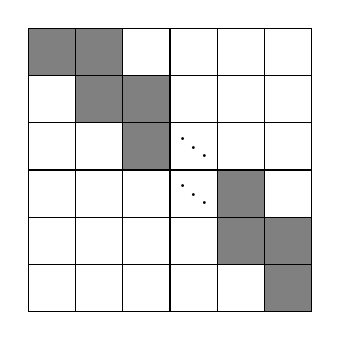
\begin{tikzpicture}[scale=0.6]
    \foreach \i/\j in {1/5, 2/5, 2/4, 3/4, 3/3, 5/2, 5/1, 6/1, 6/0} { \fill[gray] (\i, \j) rectangle (\i + 1, \j + 1); }
    \node at (4.5,3.65) {$\ddots$};
    \node at (4.5,2.65) {$\ddots$};
    \draw (1,0) grid (7,6);
  \end{tikzpicture}
  ~
  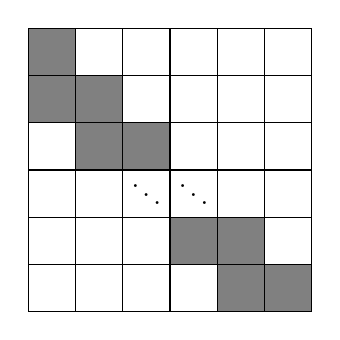
\begin{tikzpicture}[scale=0.6]
    \foreach \i/\j in {1/5, 1/4, 2/4, 2/3, 3/3, 4/1, 5/1, 5/0, 6/0} { \fill[gray] (\i, \j) rectangle (\i + 1, \j + 1); }
    \node at (3.5,2.65) {$\ddots$};
    \node at (4.5,2.65) {$\ddots$};
    \draw (1,0) grid (7,6);
  \end{tikzpicture}
  ~
  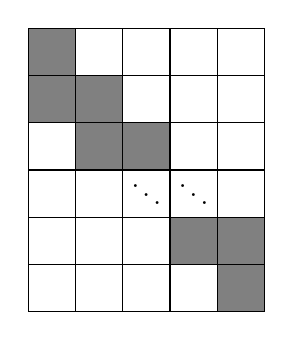
\begin{tikzpicture}[scale=0.6]
    \foreach \i/\j in {1/4, 1/5, 2/3, 2/4, 3/3, 4/1, 5/0, 5/1} { \fill[gray] (\i, \j) rectangle (\i + 1, \j + 1); }
    \node at (3.5,2.65) {$\ddots$};
    \node at (4.5,2.65) {$\ddots$};
    \draw (1,0) grid (6,6);
  \end{tikzpicture}
  ~
  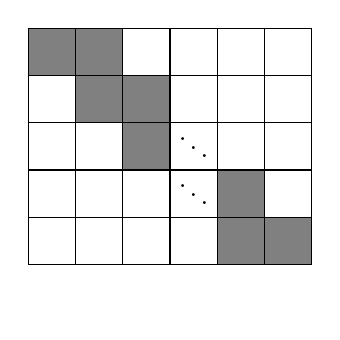
\begin{tikzpicture}[scale=0.6]
    \foreach \i/\j in {1/5, 2/5, 2/4, 3/4, 3/3, 5/2, 5/1, 6/1} { \fill[gray] (\i, \j) rectangle (\i + 1, \j + 1); }
    \node at (4.5,3.65) {$\ddots$};
    \node at (4.5,2.65) {$\ddots$};
    \path (1,0) grid (7,6);
    \draw (1,1) grid (7,6);
  \end{tikzpicture}
  \caption[Block shapes for a m\'enage permutation.]{
    Four boards, two $n \times n$ board with $2n - 1$ grey cells,
    a $n \times n-1$ board with $2n - 2$ grey cells, and a
    $n-1 \times n$ board with $2n - 2$ grey cells.
    We call them $A_n$, $A^\top_n$, $B_n$, and $B^\top_n$ respectively.
  }
  \label{fig:blockShape}
\end{figure}
